% Options for packages loaded elsewhere
\PassOptionsToPackage{unicode}{hyperref}
\PassOptionsToPackage{hyphens}{url}
%
\documentclass[
]{book}
\usepackage{amsmath,amssymb}
\usepackage{iftex}
\ifPDFTeX
  \usepackage[T1]{fontenc}
  \usepackage[utf8]{inputenc}
  \usepackage{textcomp} % provide euro and other symbols
\else % if luatex or xetex
  \usepackage{unicode-math} % this also loads fontspec
  \defaultfontfeatures{Scale=MatchLowercase}
  \defaultfontfeatures[\rmfamily]{Ligatures=TeX,Scale=1}
\fi
\usepackage{lmodern}
\ifPDFTeX\else
  % xetex/luatex font selection
\fi
% Use upquote if available, for straight quotes in verbatim environments
\IfFileExists{upquote.sty}{\usepackage{upquote}}{}
\IfFileExists{microtype.sty}{% use microtype if available
  \usepackage[]{microtype}
  \UseMicrotypeSet[protrusion]{basicmath} % disable protrusion for tt fonts
}{}
\makeatletter
\@ifundefined{KOMAClassName}{% if non-KOMA class
  \IfFileExists{parskip.sty}{%
    \usepackage{parskip}
  }{% else
    \setlength{\parindent}{0pt}
    \setlength{\parskip}{6pt plus 2pt minus 1pt}}
}{% if KOMA class
  \KOMAoptions{parskip=half}}
\makeatother
\usepackage{xcolor}
\usepackage{color}
\usepackage{fancyvrb}
\newcommand{\VerbBar}{|}
\newcommand{\VERB}{\Verb[commandchars=\\\{\}]}
\DefineVerbatimEnvironment{Highlighting}{Verbatim}{commandchars=\\\{\}}
% Add ',fontsize=\small' for more characters per line
\usepackage{framed}
\definecolor{shadecolor}{RGB}{248,248,248}
\newenvironment{Shaded}{\begin{snugshade}}{\end{snugshade}}
\newcommand{\AlertTok}[1]{\textcolor[rgb]{0.94,0.16,0.16}{#1}}
\newcommand{\AnnotationTok}[1]{\textcolor[rgb]{0.56,0.35,0.01}{\textbf{\textit{#1}}}}
\newcommand{\AttributeTok}[1]{\textcolor[rgb]{0.13,0.29,0.53}{#1}}
\newcommand{\BaseNTok}[1]{\textcolor[rgb]{0.00,0.00,0.81}{#1}}
\newcommand{\BuiltInTok}[1]{#1}
\newcommand{\CharTok}[1]{\textcolor[rgb]{0.31,0.60,0.02}{#1}}
\newcommand{\CommentTok}[1]{\textcolor[rgb]{0.56,0.35,0.01}{\textit{#1}}}
\newcommand{\CommentVarTok}[1]{\textcolor[rgb]{0.56,0.35,0.01}{\textbf{\textit{#1}}}}
\newcommand{\ConstantTok}[1]{\textcolor[rgb]{0.56,0.35,0.01}{#1}}
\newcommand{\ControlFlowTok}[1]{\textcolor[rgb]{0.13,0.29,0.53}{\textbf{#1}}}
\newcommand{\DataTypeTok}[1]{\textcolor[rgb]{0.13,0.29,0.53}{#1}}
\newcommand{\DecValTok}[1]{\textcolor[rgb]{0.00,0.00,0.81}{#1}}
\newcommand{\DocumentationTok}[1]{\textcolor[rgb]{0.56,0.35,0.01}{\textbf{\textit{#1}}}}
\newcommand{\ErrorTok}[1]{\textcolor[rgb]{0.64,0.00,0.00}{\textbf{#1}}}
\newcommand{\ExtensionTok}[1]{#1}
\newcommand{\FloatTok}[1]{\textcolor[rgb]{0.00,0.00,0.81}{#1}}
\newcommand{\FunctionTok}[1]{\textcolor[rgb]{0.13,0.29,0.53}{\textbf{#1}}}
\newcommand{\ImportTok}[1]{#1}
\newcommand{\InformationTok}[1]{\textcolor[rgb]{0.56,0.35,0.01}{\textbf{\textit{#1}}}}
\newcommand{\KeywordTok}[1]{\textcolor[rgb]{0.13,0.29,0.53}{\textbf{#1}}}
\newcommand{\NormalTok}[1]{#1}
\newcommand{\OperatorTok}[1]{\textcolor[rgb]{0.81,0.36,0.00}{\textbf{#1}}}
\newcommand{\OtherTok}[1]{\textcolor[rgb]{0.56,0.35,0.01}{#1}}
\newcommand{\PreprocessorTok}[1]{\textcolor[rgb]{0.56,0.35,0.01}{\textit{#1}}}
\newcommand{\RegionMarkerTok}[1]{#1}
\newcommand{\SpecialCharTok}[1]{\textcolor[rgb]{0.81,0.36,0.00}{\textbf{#1}}}
\newcommand{\SpecialStringTok}[1]{\textcolor[rgb]{0.31,0.60,0.02}{#1}}
\newcommand{\StringTok}[1]{\textcolor[rgb]{0.31,0.60,0.02}{#1}}
\newcommand{\VariableTok}[1]{\textcolor[rgb]{0.00,0.00,0.00}{#1}}
\newcommand{\VerbatimStringTok}[1]{\textcolor[rgb]{0.31,0.60,0.02}{#1}}
\newcommand{\WarningTok}[1]{\textcolor[rgb]{0.56,0.35,0.01}{\textbf{\textit{#1}}}}
\usepackage{longtable,booktabs,array}
\usepackage{calc} % for calculating minipage widths
% Correct order of tables after \paragraph or \subparagraph
\usepackage{etoolbox}
\makeatletter
\patchcmd\longtable{\par}{\if@noskipsec\mbox{}\fi\par}{}{}
\makeatother
% Allow footnotes in longtable head/foot
\IfFileExists{footnotehyper.sty}{\usepackage{footnotehyper}}{\usepackage{footnote}}
\makesavenoteenv{longtable}
\usepackage{graphicx}
\makeatletter
\def\maxwidth{\ifdim\Gin@nat@width>\linewidth\linewidth\else\Gin@nat@width\fi}
\def\maxheight{\ifdim\Gin@nat@height>\textheight\textheight\else\Gin@nat@height\fi}
\makeatother
% Scale images if necessary, so that they will not overflow the page
% margins by default, and it is still possible to overwrite the defaults
% using explicit options in \includegraphics[width, height, ...]{}
\setkeys{Gin}{width=\maxwidth,height=\maxheight,keepaspectratio}
% Set default figure placement to htbp
\makeatletter
\def\fps@figure{htbp}
\makeatother
\setlength{\emergencystretch}{3em} % prevent overfull lines
\providecommand{\tightlist}{%
  \setlength{\itemsep}{0pt}\setlength{\parskip}{0pt}}
\setcounter{secnumdepth}{5}
\usepackage{booktabs}
\usepackage{amsthm}
\makeatletter
\def\thm@space@setup{%
  \thm@preskip=8pt plus 2pt minus 4pt
  \thm@postskip=\thm@preskip
}
\makeatother
\usepackage{booktabs}
\usepackage{longtable}
\usepackage{array}
\usepackage{multirow}
\usepackage{wrapfig}
\usepackage{float}
\usepackage{colortbl}
\usepackage{pdflscape}
\usepackage{tabu}
\usepackage{threeparttable}
\usepackage{threeparttablex}
\usepackage[normalem]{ulem}
\usepackage{makecell}
\usepackage{xcolor}
\ifLuaTeX
  \usepackage{selnolig}  % disable illegal ligatures
\fi
\usepackage[]{natbib}
\bibliographystyle{apalike}
\IfFileExists{bookmark.sty}{\usepackage{bookmark}}{\usepackage{hyperref}}
\IfFileExists{xurl.sty}{\usepackage{xurl}}{} % add URL line breaks if available
\urlstyle{same}
\hypersetup{
  pdftitle={Introduction to Theoretical Ecology},
  pdfauthor={Instructor: Po-Ju Ke \textasciitilde\textasciitilde\textasciitilde\textasciitilde\textasciitilde{} Teaching Assistant: Guan-Yu Chen},
  hidelinks,
  pdfcreator={LaTeX via pandoc}}

\title{Introduction to Theoretical Ecology}
\author{Instructor: Po-Ju Ke \(~~~~~\) Teaching Assistant: Guan-Yu Chen}
\date{2025 Fall at National Taiwan Univeristy \includegraphics{./bifurcation.gif}}

\begin{document}
\maketitle

{
\setcounter{tocdepth}{1}
\tableofcontents
}
\hypertarget{course-information}{%
\chapter*{Course information}\label{course-information}}
\addcontentsline{toc}{chapter}{Course information}

\textbf{Description}

The development of theory plays an important role in advancing ecology as a scientific field. This three-unit course is for students at the graduate or advanced undergraduate level. The course will cover classic theoretical topics in population and community ecology, staring from single-species dynamics and gradually build up to multispecies models. Emphasis will be on theoretical concepts and corresponding mathematical approaches.

This course is designed as a two-hour lecture (written on black board) followed by a one-hour complementary hands-on practice module. In the lecture, we will analyze dynamical models and discuss their theoretical implications. In the practice section, we will use a combination interactive applications and numerical simulations to gain more intuition of the dynamics and behavior of different models.

\textbf{Objective}

By the end of the course, students are expected to be familiar with the basic building blocks of ecological models, and would be able to formulate and analyze simple models of their own. The hands-on practice component should allow students to link their ecological intuition with the underlying mathematical model, helping them to better understand the primary literature of theoretical ecology.

\textbf{Requirement}

Students are only expected to have a basic understanding of \textbf{Calculus} (e.g., freshman introductory course) and \textbf{Ecology}. It's OK if you're not familiar with calculus as we will provide relevant material for you to review during the first week.

\textbf{Format}

Thursday 6,7,8 (1:20 pm \textasciitilde{} 4:20 pm) at Gongtong 207

\textbf{Grading}

The final grade consists of:

\begin{enumerate}
\def\labelenumi{(\arabic{enumi})}
\tightlist
\item
  Assignment problem sets (60\%)
\item
  Midterm exam (15\%)
\item
  Final exam (15\%)
\item
  Course participation (10\%)
\end{enumerate}

\textbf{Course materials}

We will use a combination of textbooks of theoretical ecology. Textbook chapters and additional reading materials (listed in the course outline) will be provided. (see \href{https://pojuke.github.io/TheoreticalEcologyPJK/syllabus.html}{\textbf{Syllabus}} for more details).

Below are the textbook references:

\begin{enumerate}
\def\labelenumi{(\arabic{enumi})}
\tightlist
\item
  \emph{A Primer of Ecology} (4\textsuperscript{th} edition). Nicholas Gotelli, 2008.
\item
  \emph{An Illustrated Guide to Theoretical Ecology}. Ted Case, 2000.
\item
  \emph{A Biologist's Guide to Mathematical Modeling in Ecology and Evolution}. Sarah Otto \& Troy Day, 2011.
\item
  \emph{Mathematical Ecology of Populations and Ecosystems}. John Pastor, 2008.
\item
  \emph{Nonlinear Dynamics and Choas}. Steven Strogatz, 2000.
\end{enumerate}

\textbf{Contacts}

\textbf{Instructor}: Po-Ju Ke

\begin{itemize}
\tightlist
\item
  Office: Life Science Building R635
\item
  Email: \href{mailto:pojuke@ntu.edu.tw}{\nolinkurl{pojuke@ntu.edu.tw}}
\item
  Office hours: by appointment
\end{itemize}

\textbf{Teaching assistant}: Guan-Yu Chen

\begin{itemize}
\tightlist
\item
  Office: Life Science Building R635
\item
  Email: \href{mailto:r13b44005@ntu.edu.tw}{\nolinkurl{r13b44005@ntu.edu.tw}}
\item
  Office hours: by appointment
\end{itemize}

\hypertarget{syllabus}{%
\chapter*{Syllabus}\label{syllabus}}
\addcontentsline{toc}{chapter}{Syllabus}

\begingroup\fontsize{17}{19}\selectfont

\begin{tabu} to \linewidth {>{\centering}X>{\centering}X>{\centering}X>{\raggedright}X}
\hline
\begingroup\fontsize{20}{22}\selectfont \textcolor{black}{\textbf{Date}}\endgroup & \begingroup\fontsize{20}{22}\selectfont \textcolor{black}{\textbf{Lecture topic}}\endgroup & \begingroup\fontsize{20}{22}\selectfont \textcolor{black}{\textbf{Lab}}\endgroup & \begingroup\fontsize{20}{22}\selectfont \textcolor{black}{\textbf{Readings}}\endgroup\\
\hline
**Week 1** <span style='vertical-align:-30%'> </span>
           <br> 9/4 & Introduction: what is theoretical ecology? & \- & [**Grainger et al., 2021**](https://doi.org/10.1086/717206)\\
\hline
**Week 2** <span style='vertical-align:-30%'> </span>
           <br> 9/11 & Exponential population growth & Solving exponential growth equation using "deSolve" & Visualization & Gotelli [Ch.1], Case[Ch.1]\\
\hline
**Week 3** <span style='vertical-align:-30%'> </span>
           <br> 9/18 & Logistic population growth and stability analysis & Simulating logistic growth & \-\\
\hline
**Week 4** <span style='vertical-align:-30%'> </span>
           <br> 9/25 & Discrete population growth and stability analysis & Logistic map and Ricker diagram & Gotelli [Ch.2], Case[Ch.5], Otto & Day[Ch.5],
               [**May., 1976**](https://doi.org/10.1038/261459a0)\\
\hline
**Week 5** <span style='vertical-align:-30%'> </span>
           <br> 10/2 & Metapopulations and patch occupancy models & Metapopulations and patch occupancy models & Gotelli [Ch.4], Case[Ch.16]\\
\hline
**Week 6** <span style='vertical-align:-30%'> </span>
           <br> 10/9 & Harvesting and bifurcation & Bifurcation diagram & Pastor [Ch. 7], Strogatz [Ch. 3]\\
\hline
**Week 7** <span style='vertical-align:-30%'> </span>
           <br> 10/16 & Age-structured population models & Age-structured population model & Gotelli [Ch.3], Case[Ch.3]\\
\hline
**Week 8** <span style='vertical-align:-30%'> </span>
           <br> 10/23 & Lotka-Volterra model of competition: graphical analysis & Simulating competitive dynamics and invasion growth & Gotelli [Ch.5], Case[Ch.14], 
               [**Broekman et al., 2019**]( https://doi.org/10.1111/ele.13349)\\
\hline
**Week 9** <span style='vertical-align:-30%'> </span>
           <br> 10/30 & **Midterm exam** & \- & \-\\
\hline
**Week 10** <span style='vertical-align:-30%'> </span>
           <br> 11/6 & Lotka-Volterra model of competition: invasion analysis and linear stability analysis & Visualization of dynamics with complex eigenvalues & Otto & Day [Ch.8],
               [**May., 1972**](https://www.nature.com/articles/238413a0)\\
\hline
**Week 11** <span style='vertical-align:-30%'> </span>
           <br> 11/13 & Predator-prey interactions (I) & Lotka-Volterra model of predator-prey interactions and time-scale separation & Gotelli [Ch.6], Case[Ch.12, 13]\\
\hline
**Week 12** <span style='vertical-align:-30%'> </span>
           <br> 11/20 & Predator-prey interactions (II) & Rosenzweig-MacArthur predator-prey model & Gotelli [Ch.6], Case[Ch.12, 13]\\
\hline
**Week 13** <span style='vertical-align:-30%'> </span>
           <br> 11/27 & Multispecies models of predation: apparent competition & Consumer-resource dynamics & [**Tilman., 1980**](https://doi.org/10.1086/283633),
               [**Armstrong & McGehee., 1980**](https://doi.org/10.1086/283553)\\
\hline
**Week 14** <span style='vertical-align:-30%'> </span>
           <br> 12/4 & Mechanistic models for consumer-resource dynamics & Parameter space for apparent competition model & [**Holt., 1977**](https://doi.org/10.1016/0040-5809(77)90042-9)\\
\hline
**Week 15** <span style='vertical-align:-30%'> </span>
           <br> 12/11 & Research applcations: plant-soil feedback as an example & \- & \-\\
\hline
**Week 16** <span style='vertical-align:-30%'> </span>
           <br> 12/18 & **Final exam** & \- & \-\\
\hline
\end{tabu}
\endgroup{}

\hypertarget{week-2---exponential-population-growth}{%
\chapter*{Week 2 - Exponential population growth}\label{week-2---exponential-population-growth}}
\addcontentsline{toc}{chapter}{Week 2 - Exponential population growth}

In part 1, we will solve the differential equation for exponential population growth and visualize how the population sizes change over time.

\textbf{Part 1 - Numerical solution using the package \texttt{deSolve}}

Two main phases:

\begin{enumerate}
\def\labelenumi{(\arabic{enumi})}
\item
  Model specification: specify the structure of differential equation model
\item
  Model application: set the time steps, initial population size and model parameters (e.g., intrinsic population growth rate \(r\)), and then solve the equation model
\end{enumerate}

Consider the model
\[
\frac{dN}{dt} = rN
\]
where \(N\) is population size and \(r\) is the intrinsic growth rate.

\begin{Shaded}
\begin{Highlighting}[]
\DocumentationTok{\#\#\#\#\#\# part 1 \#\#\#\#\#\#}
\CommentTok{\# install.packages("deSolve")}
\FunctionTok{library}\NormalTok{(deSolve)}

\DocumentationTok{\#\#\# (1) Model specification}
\NormalTok{exponential\_model }\OtherTok{\textless{}{-}} \ControlFlowTok{function}\NormalTok{(times, state, parms) \{}
  \FunctionTok{with}\NormalTok{(}\FunctionTok{as.list}\NormalTok{(}\FunctionTok{c}\NormalTok{(state, parms)), \{}
\NormalTok{    dN\_dt }\OtherTok{=}\NormalTok{ r}\SpecialCharTok{*}\NormalTok{N  }\CommentTok{\# Exponential growth equation}
    \FunctionTok{return}\NormalTok{(}\FunctionTok{list}\NormalTok{(}\FunctionTok{c}\NormalTok{(dN\_dt)))  }\CommentTok{\# Return the results}
\NormalTok{  \})}
\NormalTok{\}}
\end{Highlighting}
\end{Shaded}

Set the time steps, initial population size and model parameters.

\begin{Shaded}
\begin{Highlighting}[]
\DocumentationTok{\#\#\# (2) Model application}
\NormalTok{times }\OtherTok{\textless{}{-}} \FunctionTok{seq}\NormalTok{(}\DecValTok{0}\NormalTok{, }\DecValTok{10}\NormalTok{, }\AttributeTok{by =} \FloatTok{0.1}\NormalTok{)  }\CommentTok{\# Time steps to integrate over}
\NormalTok{state }\OtherTok{\textless{}{-}} \FunctionTok{c}\NormalTok{(}\AttributeTok{N =} \DecValTok{10}\NormalTok{)  }\CommentTok{\# Initial population size}
\NormalTok{parms }\OtherTok{\textless{}{-}} \FunctionTok{c}\NormalTok{(}\AttributeTok{r =} \FloatTok{1.5}\NormalTok{)  }\CommentTok{\# Intrinsic growth rate}
\end{Highlighting}
\end{Shaded}

Solve the equation by \texttt{ode()} numerically.

\begin{Shaded}
\begin{Highlighting}[]
\CommentTok{\# Run the ode solver}
\NormalTok{pop\_size }\OtherTok{\textless{}{-}} \FunctionTok{ode}\NormalTok{(}\AttributeTok{func =}\NormalTok{ exponential\_model, }\AttributeTok{times =}\NormalTok{ times, }\AttributeTok{y =}\NormalTok{ state, }\AttributeTok{parms =}\NormalTok{ parms)}

\CommentTok{\# Take a look at the results}
\FunctionTok{head}\NormalTok{(pop\_size)}
\end{Highlighting}
\end{Shaded}

\begin{verbatim}
##      time        N
## [1,]  0.0 10.00000
## [2,]  0.1 11.61834
## [3,]  0.2 13.49860
## [4,]  0.3 15.68313
## [5,]  0.4 18.22120
## [6,]  0.5 21.17002
\end{verbatim}

Visualization

\begin{Shaded}
\begin{Highlighting}[]
\FunctionTok{plot}\NormalTok{(N }\SpecialCharTok{\textasciitilde{}}\NormalTok{ time, }\AttributeTok{data =}\NormalTok{ pop\_size)}
\end{Highlighting}
\end{Shaded}

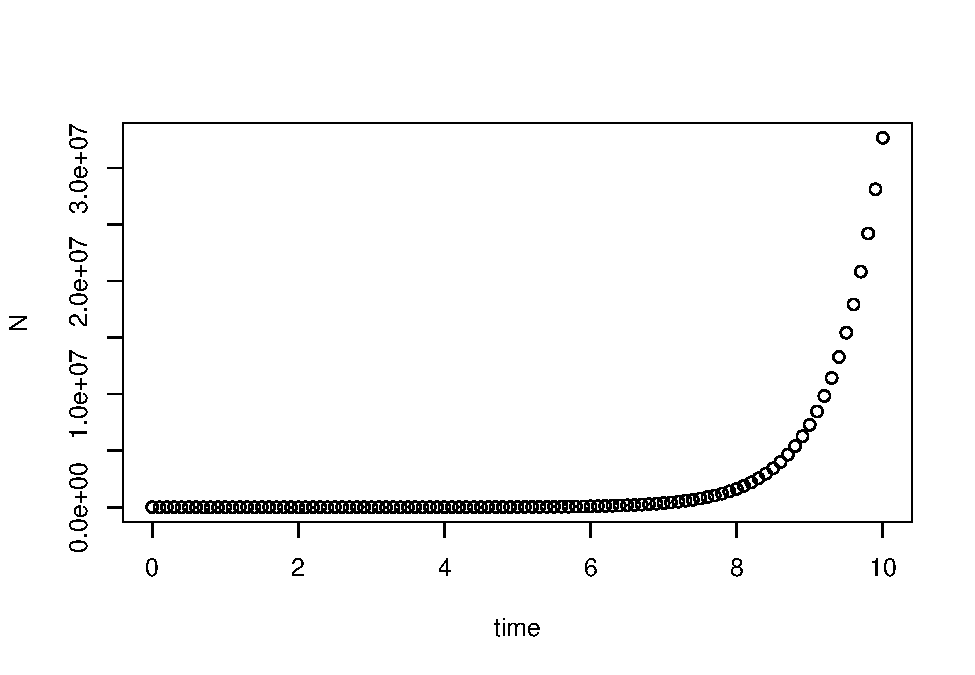
\includegraphics{bookdown-demo_files/figure-latex/unnamed-chunk-5-1.pdf}

Compare simulation result with analytic solution, which is
\[
N(t) = N_0\exp\{rt\}
\]

\begin{Shaded}
\begin{Highlighting}[]
\FunctionTok{par}\NormalTok{(}\AttributeTok{mfrow =} \FunctionTok{c}\NormalTok{(}\DecValTok{1}\NormalTok{,}\DecValTok{2}\NormalTok{))}
\FunctionTok{plot}\NormalTok{(N }\SpecialCharTok{\textasciitilde{}}\NormalTok{ time, }\AttributeTok{data =}\NormalTok{ pop\_size) }\CommentTok{\# Plot simulation data}
\FunctionTok{curve}\NormalTok{(state[}\DecValTok{1}\NormalTok{]}\SpecialCharTok{*}\FunctionTok{exp}\NormalTok{(parms[}\DecValTok{1}\NormalTok{]}\SpecialCharTok{*}\NormalTok{x), }\AttributeTok{col =} \StringTok{"red"}\NormalTok{, }\AttributeTok{add =}\NormalTok{ T) }\CommentTok{\# Adding analytic solution}
\FunctionTok{plot}\NormalTok{(N }\SpecialCharTok{\textasciitilde{}}\NormalTok{ time, }\AttributeTok{data =}\NormalTok{ pop\_size, }\AttributeTok{log =} \StringTok{"y"}\NormalTok{) }\CommentTok{\# Plot logged simulation data}
\FunctionTok{curve}\NormalTok{(state[}\DecValTok{1}\NormalTok{]}\SpecialCharTok{*}\FunctionTok{exp}\NormalTok{(parms[}\DecValTok{1}\NormalTok{]}\SpecialCharTok{*}\NormalTok{x), }\AttributeTok{col =} \StringTok{"red"}\NormalTok{, }\AttributeTok{add =}\NormalTok{ T) }\CommentTok{\# Adding analytic solution}
\end{Highlighting}
\end{Shaded}

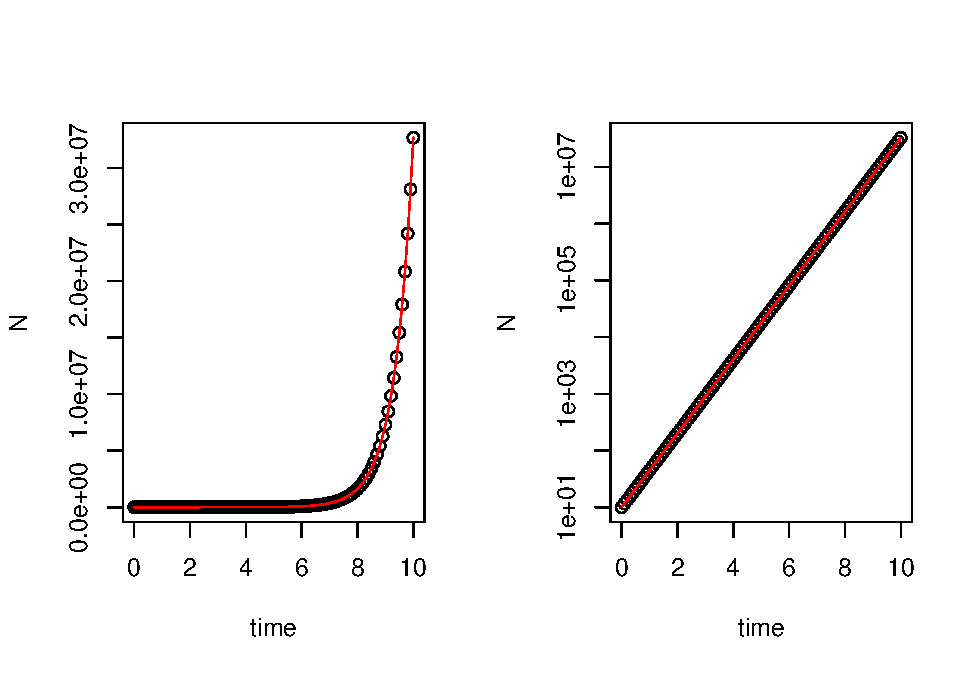
\includegraphics{bookdown-demo_files/figure-latex/unnamed-chunk-6-1.pdf}

\textbf{Part 2 - Comparing different ode solvers and different time intervals}
In default of \texttt{ode()}, the equations are solved by LSODA method. We can change the method by modifying the argument \texttt{method} in \texttt{ode()}.

\begin{Shaded}
\begin{Highlighting}[]
\DocumentationTok{\#\#\#\#\#\# part 2 \#\#\#\#\#\#}
\CommentTok{\# Original setting}
\NormalTok{times }\OtherTok{\textless{}{-}} \FunctionTok{seq}\NormalTok{(}\DecValTok{0}\NormalTok{, }\DecValTok{10}\NormalTok{, }\AttributeTok{by =} \FloatTok{0.1}\NormalTok{)  }\CommentTok{\# Time steps to integrate over}
\NormalTok{state }\OtherTok{\textless{}{-}} \FunctionTok{c}\NormalTok{(}\AttributeTok{N =} \DecValTok{10}\NormalTok{)  }\CommentTok{\# Initial population size}
\NormalTok{parms }\OtherTok{\textless{}{-}} \FunctionTok{c}\NormalTok{(}\AttributeTok{r =} \FloatTok{1.5}\NormalTok{)  }\CommentTok{\# Intrinsic growth rate}
\CommentTok{\# Default: LSODA}
\NormalTok{pop\_size }\OtherTok{\textless{}{-}} \FunctionTok{ode}\NormalTok{(}\AttributeTok{func =}\NormalTok{ exponential\_model, }\AttributeTok{times =}\NormalTok{ times, }\AttributeTok{y =}\NormalTok{ state, }\AttributeTok{parms =}\NormalTok{ parms)}

\CommentTok{\# Euler\textquotesingle{}s method}
\NormalTok{pop\_size\_1 }\OtherTok{\textless{}{-}} \FunctionTok{ode}\NormalTok{(}\AttributeTok{func =}\NormalTok{ exponential\_model, }\AttributeTok{times =}\NormalTok{ times, }\AttributeTok{y =}\NormalTok{ state, }\AttributeTok{parms =}\NormalTok{ parms, }\AttributeTok{method =} \StringTok{"euler"}\NormalTok{)}

\CommentTok{\# Compare different method}
\FunctionTok{par}\NormalTok{(}\AttributeTok{mfrow =} \FunctionTok{c}\NormalTok{(}\DecValTok{1}\NormalTok{,}\DecValTok{2}\NormalTok{))}
\FunctionTok{plot}\NormalTok{(N }\SpecialCharTok{\textasciitilde{}}\NormalTok{ time, }\AttributeTok{data =}\NormalTok{ pop\_size, }\AttributeTok{main =} \StringTok{"LSODA"}\NormalTok{)}
\FunctionTok{curve}\NormalTok{(state[}\DecValTok{1}\NormalTok{]}\SpecialCharTok{*}\FunctionTok{exp}\NormalTok{(parms[}\DecValTok{1}\NormalTok{]}\SpecialCharTok{*}\NormalTok{x), times[}\DecValTok{1}\NormalTok{], times[}\FunctionTok{length}\NormalTok{(times)], }\AttributeTok{col =} \StringTok{"red"}\NormalTok{, }\AttributeTok{add =}\NormalTok{ T) }\CommentTok{\# correct curve}
\FunctionTok{plot}\NormalTok{(N }\SpecialCharTok{\textasciitilde{}}\NormalTok{ time, }\AttributeTok{data =}\NormalTok{ pop\_size\_1, }\AttributeTok{main =} \StringTok{"Euler"}\NormalTok{)}
\FunctionTok{curve}\NormalTok{(state[}\DecValTok{1}\NormalTok{]}\SpecialCharTok{*}\FunctionTok{exp}\NormalTok{(parms[}\DecValTok{1}\NormalTok{]}\SpecialCharTok{*}\NormalTok{x), times[}\DecValTok{1}\NormalTok{], times[}\FunctionTok{length}\NormalTok{(times)], }\AttributeTok{col =} \StringTok{"red"}\NormalTok{, }\AttributeTok{add =}\NormalTok{ T) }\CommentTok{\# correct curve}
\end{Highlighting}
\end{Shaded}

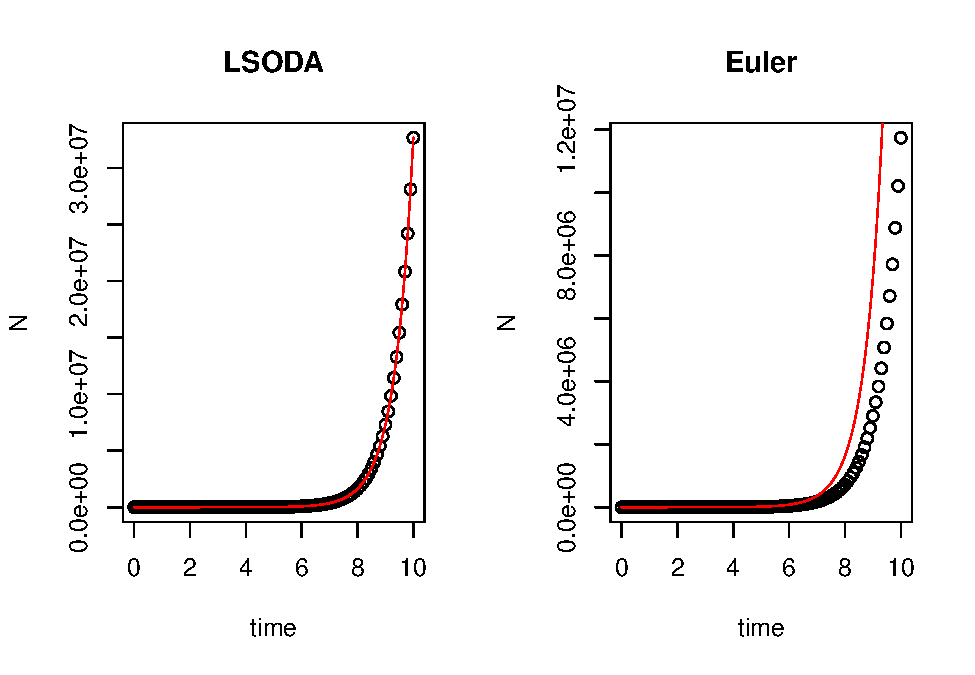
\includegraphics{bookdown-demo_files/figure-latex/unnamed-chunk-7-1.pdf}

\begin{Shaded}
\begin{Highlighting}[]
\CommentTok{\# Different time intervals}
\NormalTok{times\_1 }\OtherTok{\textless{}{-}} \FunctionTok{seq}\NormalTok{(}\DecValTok{0}\NormalTok{, }\DecValTok{10}\NormalTok{, }\AttributeTok{by =} \DecValTok{1}\NormalTok{)  }\CommentTok{\# time steps to integrate over}
\NormalTok{times\_2 }\OtherTok{\textless{}{-}} \FunctionTok{seq}\NormalTok{(}\DecValTok{0}\NormalTok{, }\DecValTok{10}\NormalTok{, }\AttributeTok{by =} \FloatTok{0.1}\NormalTok{)  }\CommentTok{\# time steps to integrate over}
\NormalTok{times\_3 }\OtherTok{\textless{}{-}} \FunctionTok{seq}\NormalTok{(}\DecValTok{0}\NormalTok{, }\DecValTok{10}\NormalTok{, }\AttributeTok{by =} \FloatTok{0.01}\NormalTok{)  }\CommentTok{\# time steps to integrate over}

\CommentTok{\# Euler\textquotesingle{}s method}
\NormalTok{pop\_size\_1 }\OtherTok{\textless{}{-}} \FunctionTok{ode}\NormalTok{(}\AttributeTok{func =}\NormalTok{ exponential\_model, }\AttributeTok{times =}\NormalTok{ times\_1, }\AttributeTok{y =}\NormalTok{ state, }\AttributeTok{parms =}\NormalTok{ parms, }\AttributeTok{method =} \StringTok{"euler"}\NormalTok{)}
\NormalTok{pop\_size\_2 }\OtherTok{\textless{}{-}} \FunctionTok{ode}\NormalTok{(}\AttributeTok{func =}\NormalTok{ exponential\_model, }\AttributeTok{times =}\NormalTok{ times\_2, }\AttributeTok{y =}\NormalTok{ state, }\AttributeTok{parms =}\NormalTok{ parms, }\AttributeTok{method =} \StringTok{"euler"}\NormalTok{)}
\NormalTok{pop\_size\_3 }\OtherTok{\textless{}{-}} \FunctionTok{ode}\NormalTok{(}\AttributeTok{func =}\NormalTok{ exponential\_model, }\AttributeTok{times =}\NormalTok{ times\_3, }\AttributeTok{y =}\NormalTok{ state, }\AttributeTok{parms =}\NormalTok{ parms, }\AttributeTok{method =} \StringTok{"euler"}\NormalTok{)}

\CommentTok{\# Compare different time intervals}
\FunctionTok{par}\NormalTok{(}\AttributeTok{mfrow =} \FunctionTok{c}\NormalTok{(}\DecValTok{1}\NormalTok{,}\DecValTok{3}\NormalTok{))}
\FunctionTok{plot}\NormalTok{(N }\SpecialCharTok{\textasciitilde{}}\NormalTok{ time, }\AttributeTok{data =}\NormalTok{ pop\_size\_1, }\AttributeTok{main =} \StringTok{"Time intervals = 1"}\NormalTok{)}
\FunctionTok{curve}\NormalTok{(state[}\DecValTok{1}\NormalTok{]}\SpecialCharTok{*}\FunctionTok{exp}\NormalTok{(parms[}\DecValTok{1}\NormalTok{]}\SpecialCharTok{*}\NormalTok{x), }\AttributeTok{col =} \StringTok{"red"}\NormalTok{, }\AttributeTok{add =}\NormalTok{ T) }\CommentTok{\# correct curve}
\FunctionTok{plot}\NormalTok{(N }\SpecialCharTok{\textasciitilde{}}\NormalTok{ time, }\AttributeTok{data =}\NormalTok{ pop\_size\_2, }\AttributeTok{main =} \StringTok{"Time intervals = 0.1"}\NormalTok{)}
\FunctionTok{curve}\NormalTok{(state[}\DecValTok{1}\NormalTok{]}\SpecialCharTok{*}\FunctionTok{exp}\NormalTok{(parms[}\DecValTok{1}\NormalTok{]}\SpecialCharTok{*}\NormalTok{x), }\AttributeTok{col =} \StringTok{"red"}\NormalTok{, }\AttributeTok{add =}\NormalTok{ T) }\CommentTok{\# correct curve}
\FunctionTok{plot}\NormalTok{(N }\SpecialCharTok{\textasciitilde{}}\NormalTok{ time, }\AttributeTok{data =}\NormalTok{ pop\_size\_3, }\AttributeTok{main =} \StringTok{"Time intervals = 0.01"}\NormalTok{)}
\FunctionTok{curve}\NormalTok{(state[}\DecValTok{1}\NormalTok{]}\SpecialCharTok{*}\FunctionTok{exp}\NormalTok{(parms[}\DecValTok{1}\NormalTok{]}\SpecialCharTok{*}\NormalTok{x), }\AttributeTok{col =} \StringTok{"red"}\NormalTok{, }\AttributeTok{add =}\NormalTok{ T) }\CommentTok{\# correct curve}
\end{Highlighting}
\end{Shaded}

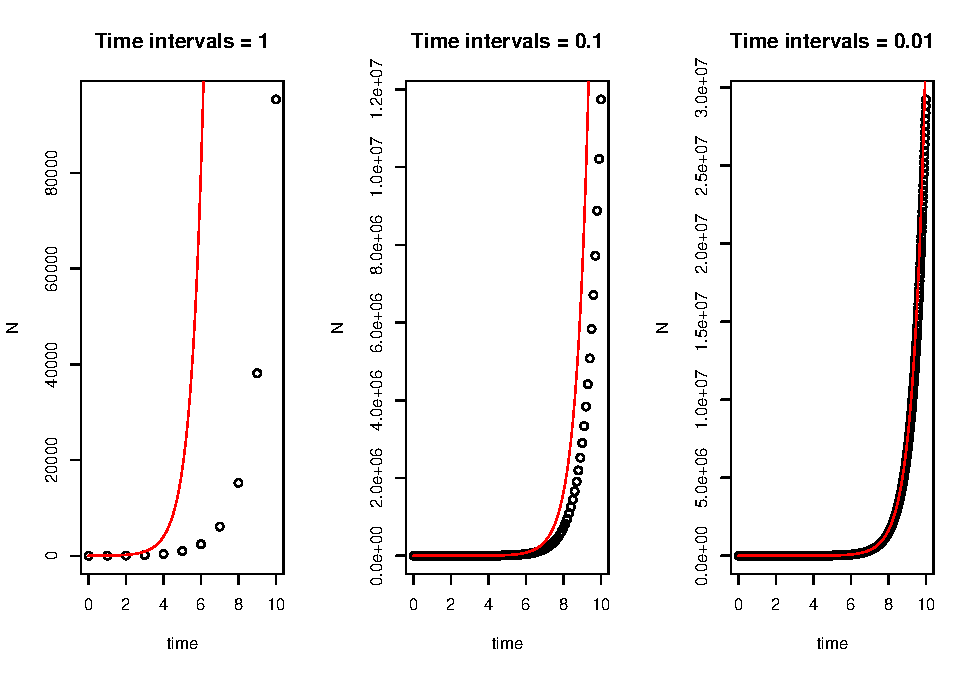
\includegraphics{bookdown-demo_files/figure-latex/unnamed-chunk-7-2.pdf}

\textbf{Part 3 - Solving exponential growth model with fluctuating growth rate}
Consider the model
\[
\frac{dN}{dt} = r(t)N \ \text{, } r(t) = \overline{r} + \sigma\sin(\omega t)
\]
where \(\overline{r}\) and \(\omega\) are constants.
The analytic solution of the ode model is
\[
N(t) = N_0\exp\{\overline{r}t - \frac{\sigma}{\omega}[\cos(\omega t) - 1]\}
\]

\begin{Shaded}
\begin{Highlighting}[]
\DocumentationTok{\#\#\#\#\#\# part 3 \#\#\#\#\#\#}
\DocumentationTok{\#\#\# Model specification}
\NormalTok{exponential\_model\_fluc }\OtherTok{\textless{}{-}} \ControlFlowTok{function}\NormalTok{(times, state, parms) \{}
  \FunctionTok{with}\NormalTok{(}\FunctionTok{as.list}\NormalTok{(}\FunctionTok{c}\NormalTok{(state, parms)), \{}
\NormalTok{    dN\_dt }\OtherTok{=}\NormalTok{ (r\_bar }\SpecialCharTok{+}\NormalTok{ sigma}\SpecialCharTok{*}\FunctionTok{sin}\NormalTok{(omega}\SpecialCharTok{*}\NormalTok{times))}\SpecialCharTok{*}\NormalTok{N  }\CommentTok{\# exponential growth equation}
    \FunctionTok{return}\NormalTok{(}\FunctionTok{list}\NormalTok{(}\FunctionTok{c}\NormalTok{(dN\_dt)))  }\CommentTok{\# return the results}
\NormalTok{  \})}
\NormalTok{\}}
\end{Highlighting}
\end{Shaded}

\begin{Shaded}
\begin{Highlighting}[]
\DocumentationTok{\#\#\# Parameters}
\NormalTok{times }\OtherTok{\textless{}{-}} \FunctionTok{seq}\NormalTok{(}\DecValTok{0}\NormalTok{, }\DecValTok{10}\NormalTok{, }\AttributeTok{by =} \FloatTok{0.1}\NormalTok{)  }\CommentTok{\# time steps to integrate over}
\NormalTok{state }\OtherTok{\textless{}{-}} \FunctionTok{c}\NormalTok{(}\AttributeTok{N =} \DecValTok{10}\NormalTok{)  }\CommentTok{\# initial population size}
\NormalTok{parms }\OtherTok{\textless{}{-}} \FunctionTok{c}\NormalTok{(}\AttributeTok{r\_bar =} \FloatTok{1.5}\NormalTok{, }\AttributeTok{sigma =} \DecValTok{5}\NormalTok{, }\AttributeTok{omega =} \DecValTok{2}\SpecialCharTok{*}\NormalTok{pi)  }\CommentTok{\# intrinsic growth rate}
\end{Highlighting}
\end{Shaded}

Plot \(r(t)\)

\begin{Shaded}
\begin{Highlighting}[]
\DocumentationTok{\#\#\# Fluctuating growth rate}
\NormalTok{r }\OtherTok{=}\NormalTok{ parms[}\DecValTok{1}\NormalTok{] }\SpecialCharTok{+}\NormalTok{ parms[}\DecValTok{2}\NormalTok{]}\SpecialCharTok{*}\FunctionTok{sin}\NormalTok{(parms[}\DecValTok{3}\NormalTok{]}\SpecialCharTok{*}\NormalTok{times)}
\FunctionTok{plot}\NormalTok{(r }\SpecialCharTok{\textasciitilde{}}\NormalTok{ times, }\AttributeTok{type =} \StringTok{"l"}\NormalTok{)}
\end{Highlighting}
\end{Shaded}

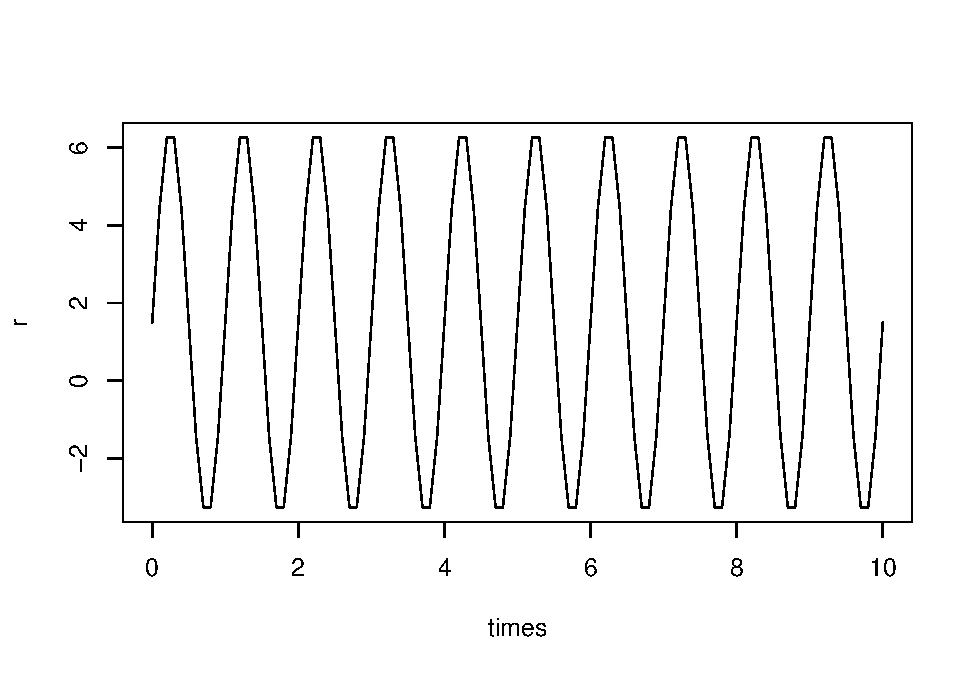
\includegraphics{bookdown-demo_files/figure-latex/unnamed-chunk-10-1.pdf}

\begin{Shaded}
\begin{Highlighting}[]
\DocumentationTok{\#\#\# Solving model}
\NormalTok{pop\_size }\OtherTok{\textless{}{-}} \FunctionTok{ode}\NormalTok{(}\AttributeTok{func =}\NormalTok{ exponential\_model\_fluc, }\AttributeTok{times =}\NormalTok{ times, }\AttributeTok{y =}\NormalTok{ state, }\AttributeTok{parms =}\NormalTok{ parms)}

\DocumentationTok{\#\#\# Plotting}
\FunctionTok{plot}\NormalTok{(N }\SpecialCharTok{\textasciitilde{}}\NormalTok{ times, }\AttributeTok{data =}\NormalTok{ pop\_size)}
\FunctionTok{curve}\NormalTok{(state[}\DecValTok{1}\NormalTok{]}\SpecialCharTok{*}\FunctionTok{exp}\NormalTok{(parms[}\DecValTok{1}\NormalTok{]}\SpecialCharTok{*}\NormalTok{x }\SpecialCharTok{{-}}\NormalTok{ parms[}\DecValTok{2}\NormalTok{]}\SpecialCharTok{/}\NormalTok{parms[}\DecValTok{3}\NormalTok{]}\SpecialCharTok{*}\NormalTok{(}\FunctionTok{cos}\NormalTok{(parms[}\DecValTok{3}\NormalTok{]}\SpecialCharTok{*}\NormalTok{x) }\SpecialCharTok{{-}} \DecValTok{1}\NormalTok{)), }\AttributeTok{add =}\NormalTok{ T, }\AttributeTok{col =} \StringTok{"red"}\NormalTok{) }\CommentTok{\# correct curve}
\end{Highlighting}
\end{Shaded}

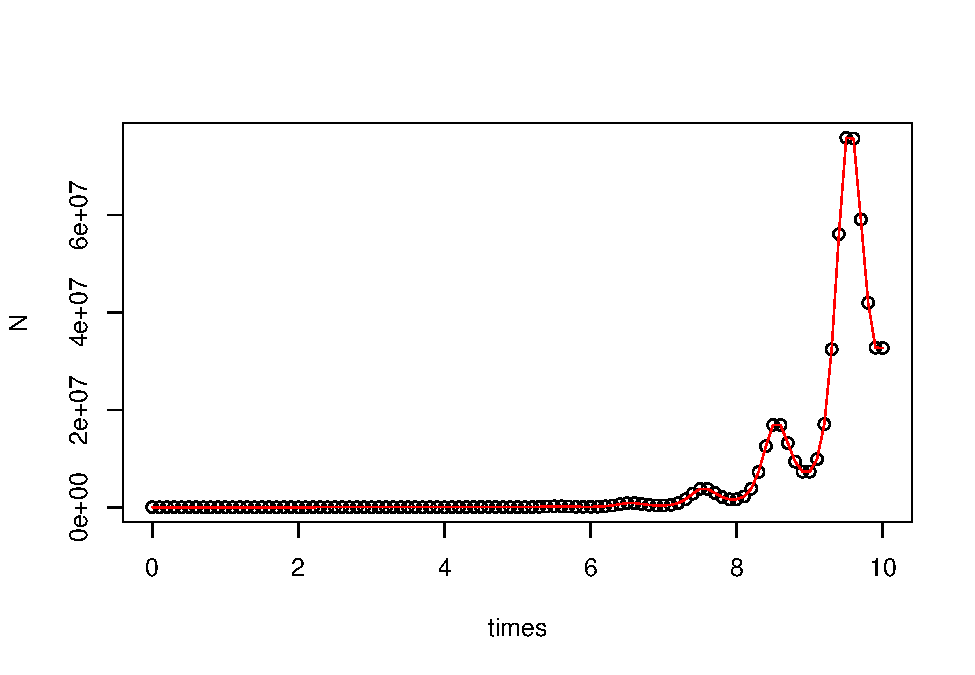
\includegraphics{bookdown-demo_files/figure-latex/unnamed-chunk-11-1.pdf}

\begin{Shaded}
\begin{Highlighting}[]
\FunctionTok{plot}\NormalTok{(N }\SpecialCharTok{\textasciitilde{}}\NormalTok{ times, }\AttributeTok{data =}\NormalTok{ pop\_size, }\AttributeTok{log =} \StringTok{"y"}\NormalTok{)}
\FunctionTok{curve}\NormalTok{(state[}\DecValTok{1}\NormalTok{]}\SpecialCharTok{*}\FunctionTok{exp}\NormalTok{(parms[}\DecValTok{1}\NormalTok{]}\SpecialCharTok{*}\NormalTok{x }\SpecialCharTok{{-}}\NormalTok{ parms[}\DecValTok{2}\NormalTok{]}\SpecialCharTok{/}\NormalTok{parms[}\DecValTok{3}\NormalTok{]}\SpecialCharTok{*}\NormalTok{(}\FunctionTok{cos}\NormalTok{(parms[}\DecValTok{3}\NormalTok{]}\SpecialCharTok{*}\NormalTok{x) }\SpecialCharTok{{-}} \DecValTok{1}\NormalTok{)), }\AttributeTok{add =}\NormalTok{ T, }\AttributeTok{col =} \StringTok{"red"}\NormalTok{) }\CommentTok{\# correct curve}
\end{Highlighting}
\end{Shaded}

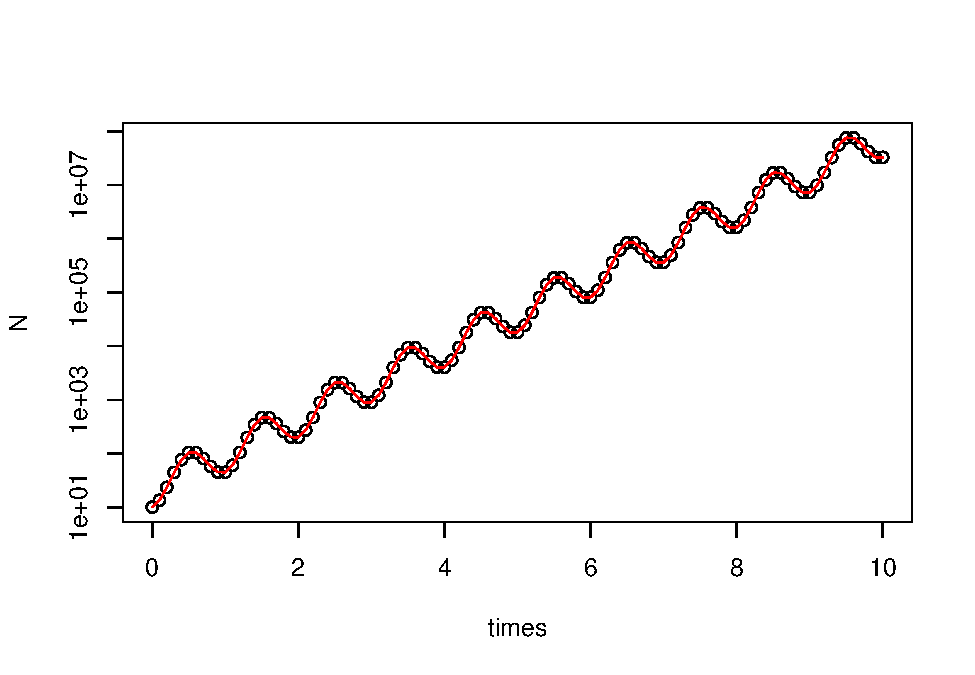
\includegraphics{bookdown-demo_files/figure-latex/unnamed-chunk-11-2.pdf}

Adjust \(\overline{r}\)

\begin{Shaded}
\begin{Highlighting}[]
\DocumentationTok{\#\#\# Parameters}
\NormalTok{times }\OtherTok{\textless{}{-}} \FunctionTok{seq}\NormalTok{(}\DecValTok{0}\NormalTok{, }\DecValTok{10}\NormalTok{, }\AttributeTok{by =} \FloatTok{0.1}\NormalTok{)  }\CommentTok{\# time steps to integrate over}
\NormalTok{state }\OtherTok{\textless{}{-}} \FunctionTok{c}\NormalTok{(}\AttributeTok{N =} \DecValTok{10}\NormalTok{)  }\CommentTok{\# initial population size}
\NormalTok{parms }\OtherTok{\textless{}{-}} \FunctionTok{c}\NormalTok{(}\AttributeTok{r\_bar =} \FloatTok{0.1}\NormalTok{, }\AttributeTok{sigma =} \DecValTok{5}\NormalTok{, }\AttributeTok{omega =} \DecValTok{2}\SpecialCharTok{*}\NormalTok{pi)  }\CommentTok{\# intrinsic growth rate}

\DocumentationTok{\#\#\# Fluctuating growth rate}
\NormalTok{r }\OtherTok{=}\NormalTok{ parms[}\DecValTok{1}\NormalTok{] }\SpecialCharTok{+}\NormalTok{ parms[}\DecValTok{2}\NormalTok{]}\SpecialCharTok{*}\FunctionTok{sin}\NormalTok{(parms[}\DecValTok{3}\NormalTok{]}\SpecialCharTok{*}\NormalTok{times)}
\FunctionTok{plot}\NormalTok{(r }\SpecialCharTok{\textasciitilde{}}\NormalTok{ times, }\AttributeTok{type =} \StringTok{"l"}\NormalTok{)}
\end{Highlighting}
\end{Shaded}

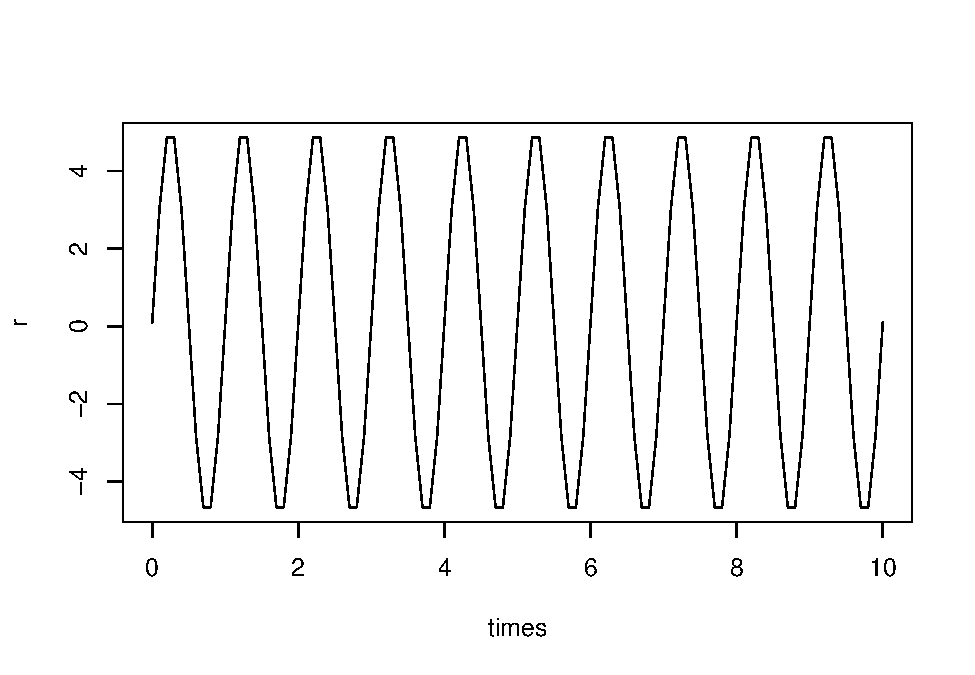
\includegraphics{bookdown-demo_files/figure-latex/unnamed-chunk-12-1.pdf}

\begin{Shaded}
\begin{Highlighting}[]
\DocumentationTok{\#\#\# Solving model}
\NormalTok{pop\_size }\OtherTok{\textless{}{-}} \FunctionTok{ode}\NormalTok{(}\AttributeTok{func =}\NormalTok{ exponential\_model\_fluc, }\AttributeTok{times =}\NormalTok{ times, }\AttributeTok{y =}\NormalTok{ state, }\AttributeTok{parms =}\NormalTok{ parms)}

\DocumentationTok{\#\#\# Plotting}
\FunctionTok{plot}\NormalTok{(N }\SpecialCharTok{\textasciitilde{}}\NormalTok{ times, }\AttributeTok{data =}\NormalTok{ pop\_size)}
\FunctionTok{curve}\NormalTok{(state[}\DecValTok{1}\NormalTok{]}\SpecialCharTok{*}\FunctionTok{exp}\NormalTok{(parms[}\DecValTok{1}\NormalTok{]}\SpecialCharTok{*}\NormalTok{x }\SpecialCharTok{{-}}\NormalTok{ parms[}\DecValTok{2}\NormalTok{]}\SpecialCharTok{/}\NormalTok{parms[}\DecValTok{3}\NormalTok{]}\SpecialCharTok{*}\NormalTok{(}\FunctionTok{cos}\NormalTok{(parms[}\DecValTok{3}\NormalTok{]}\SpecialCharTok{*}\NormalTok{x) }\SpecialCharTok{{-}} \DecValTok{1}\NormalTok{)), }\AttributeTok{add =}\NormalTok{ T, }\AttributeTok{col =} \StringTok{"red"}\NormalTok{) }\CommentTok{\# correct curve}
\end{Highlighting}
\end{Shaded}

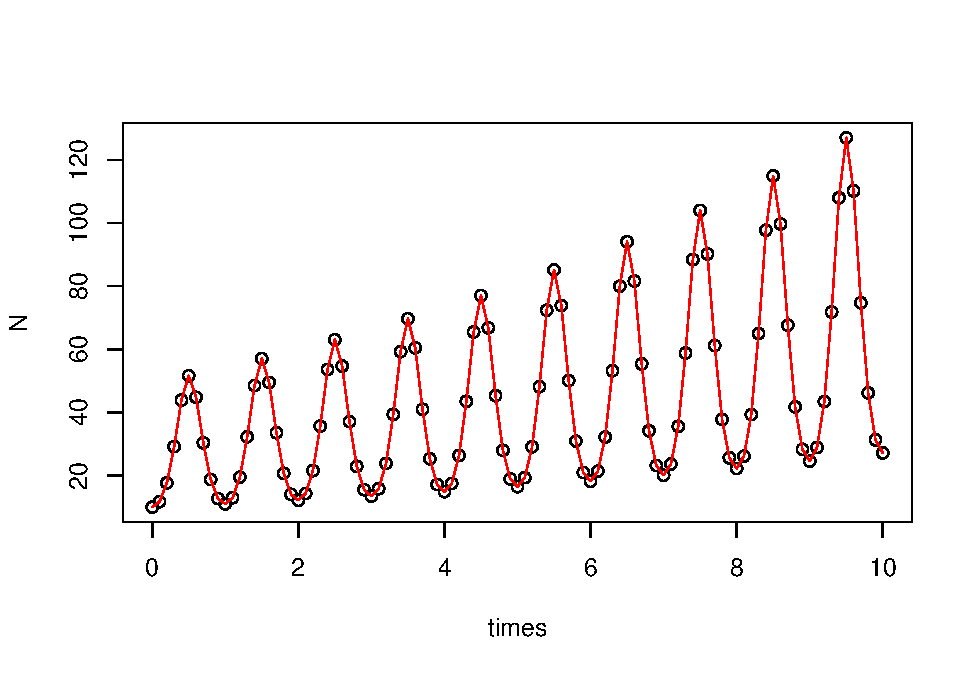
\includegraphics{bookdown-demo_files/figure-latex/unnamed-chunk-12-2.pdf}

\hypertarget{week-3---logistic-population-growth-and-stability-analysis}{%
\chapter*{Week 3 - Logistic population growth and stability analysis}\label{week-3---logistic-population-growth-and-stability-analysis}}
\addcontentsline{toc}{chapter}{Week 3 - Logistic population growth and stability analysis}

\textbf{Part 1 - Shining app for logistic growth}

Credit to \href{https://genchanghsu.github.io/index.html}{Gen-Chang Hsu}

\textbf{Part 2 - Population growth with Allee effects}

Some populations experience negative growth rates when the population size is too low, a phenomenon known as ``Allee effect''. For example, some flowering plants require a minimal local density to attract pollinators (clustering effects). Below this density, pollinators will not be able to detect the presence of flowers and therefore the plants cannot complete their life cycle. Some flower species, e.g., \emph{Itea}, requires a minimal population size of \(A\) to attract its specialized bee pollinator and its population growth is directly related to pollinator visitation, its population dynamics can be described using the below differential equation:

\[
\frac{dN}{dt} = rN(1-\frac{N}{K})(\frac{N}{A}-1)
\]

where \(0 < A < K\). The term \(A\) represents ``Allee threshold'', below which the population growth rate is negative (because of no visiting pollinators) and thus the population will decline; \(r\) is the intrinsic rate of increase and \(K\) is the carrying capacity.

\begin{enumerate}
\def\labelenumi{(\arabic{enumi})}
\tightlist
\item
  You can calculate the equilibrium population sizes and use the graphical method to determine their stability. The equilibrium population sizes are \(N^* = 0\) (stable), \(N^* = A\) (unstable), and \(N^* = K\) (stable).
\end{enumerate}

\begin{Shaded}
\begin{Highlighting}[]
\NormalTok{r }\OtherTok{=} \DecValTok{1}
\NormalTok{A }\OtherTok{=} \DecValTok{150}
\NormalTok{K }\OtherTok{=} \DecValTok{500}
\FunctionTok{curve}\NormalTok{(r}\SpecialCharTok{*}\NormalTok{x}\SpecialCharTok{*}\NormalTok{(}\DecValTok{1}\SpecialCharTok{{-}}\NormalTok{x}\SpecialCharTok{/}\NormalTok{K)}\SpecialCharTok{*}\NormalTok{(x}\SpecialCharTok{/}\NormalTok{A}\DecValTok{{-}1}\NormalTok{), }\AttributeTok{from =} \DecValTok{0}\NormalTok{, }\AttributeTok{to =} \DecValTok{550}\NormalTok{, }\AttributeTok{xlim =} \FunctionTok{c}\NormalTok{(}\DecValTok{0}\NormalTok{, }\DecValTok{550}\NormalTok{),}
      \AttributeTok{xlab =} \StringTok{"N"}\NormalTok{, }\AttributeTok{ylab =} \StringTok{"dN/dt"}\NormalTok{, }\AttributeTok{las =} \DecValTok{1}\NormalTok{)}
\FunctionTok{abline}\NormalTok{(}\AttributeTok{h =} \DecValTok{0}\NormalTok{, }\AttributeTok{lty =} \DecValTok{2}\NormalTok{)}
\FunctionTok{points}\NormalTok{(}\AttributeTok{y =} \FunctionTok{rep}\NormalTok{(}\DecValTok{0}\NormalTok{, }\DecValTok{3}\NormalTok{), }\AttributeTok{x =} \FunctionTok{c}\NormalTok{(}\DecValTok{0}\NormalTok{, A, K), }\AttributeTok{pch =} \FunctionTok{c}\NormalTok{(}\DecValTok{16}\NormalTok{, }\DecValTok{1}\NormalTok{, }\DecValTok{16}\NormalTok{))}
\FunctionTok{text}\NormalTok{(}\AttributeTok{x =} \FunctionTok{c}\NormalTok{(}\DecValTok{0}\NormalTok{, A, K), }\AttributeTok{y =} \FunctionTok{rep}\NormalTok{(}\DecValTok{20}\NormalTok{, }\DecValTok{3}\NormalTok{), }\AttributeTok{labels =} \FunctionTok{c}\NormalTok{(}\StringTok{"0"}\NormalTok{, }\StringTok{"A"}\NormalTok{, }\StringTok{"K"}\NormalTok{), }\AttributeTok{font =} \DecValTok{3}\NormalTok{, }\AttributeTok{col =} \StringTok{"blue"}\NormalTok{)}
\FunctionTok{arrows}\NormalTok{(}\AttributeTok{x0 =} \FunctionTok{c}\NormalTok{(}\DecValTok{100}\NormalTok{, }\DecValTok{200}\NormalTok{, }\DecValTok{550}\NormalTok{), }\AttributeTok{y0 =} \SpecialCharTok{{-}}\DecValTok{10}\NormalTok{, }\AttributeTok{x1 =} \FunctionTok{c}\NormalTok{(}\DecValTok{10}\NormalTok{, }\DecValTok{450}\NormalTok{, }\DecValTok{510}\NormalTok{), }\AttributeTok{y1 =} \SpecialCharTok{{-}}\DecValTok{10}\NormalTok{, }\AttributeTok{length =} \FloatTok{0.08}\NormalTok{, }\AttributeTok{lwd =} \DecValTok{2}\NormalTok{)}
\end{Highlighting}
\end{Shaded}

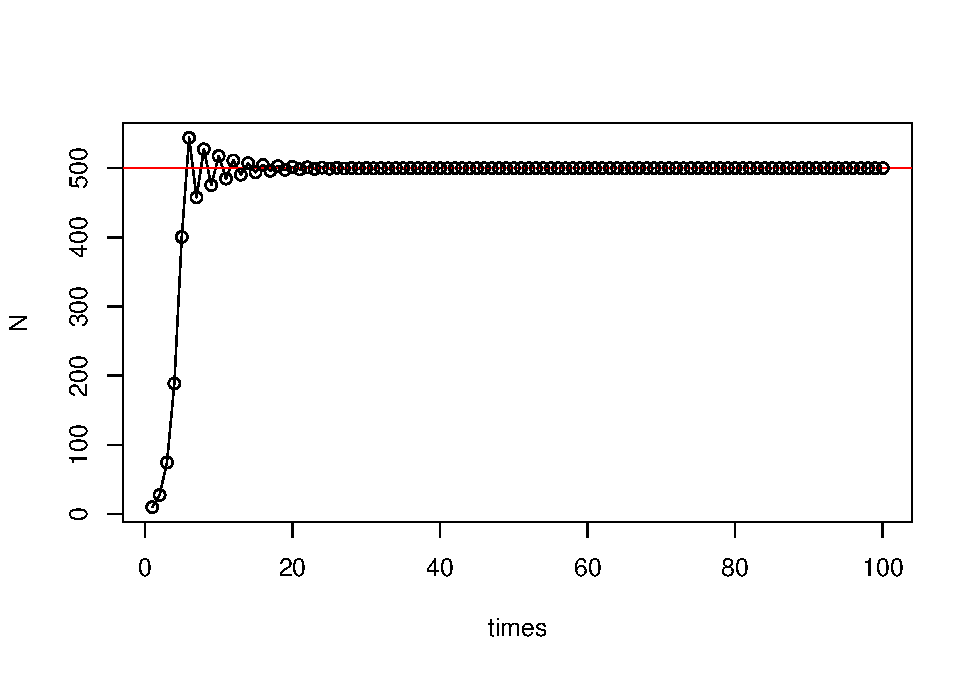
\includegraphics{bookdown-demo_files/figure-latex/unnamed-chunk-14-1.pdf}

\begin{enumerate}
\def\labelenumi{(\arabic{enumi})}
\setcounter{enumi}{1}
\tightlist
\item
  Simulate the dynamics with an intrinsic rate of increase of \(r\) = 1.2, the carrying capacity of \(K\) = 1000, and the minimal threshold density of \(A\) = 150. Observe the population trajectories to see how different initial population sizes can lead to different equilibrium population sizes (a phenomenon known as ``alternative stable states'').
\end{enumerate}

\begin{Shaded}
\begin{Highlighting}[]
\FunctionTok{library}\NormalTok{(deSolve)}
\NormalTok{Allee }\OtherTok{\textless{}{-}} \ControlFlowTok{function}\NormalTok{(t, state, pars) \{}
  \FunctionTok{with}\NormalTok{(}\FunctionTok{as.list}\NormalTok{(}\FunctionTok{c}\NormalTok{(state, pars)), \{}
\NormalTok{    dN\_dt }\OtherTok{=}\NormalTok{ r}\SpecialCharTok{*}\NormalTok{N}\SpecialCharTok{*}\NormalTok{(}\DecValTok{1}\SpecialCharTok{{-}}\NormalTok{N}\SpecialCharTok{/}\NormalTok{K)}\SpecialCharTok{*}\NormalTok{(N}\SpecialCharTok{/}\NormalTok{A}\DecValTok{{-}1}\NormalTok{)}
    \FunctionTok{return}\NormalTok{(}\FunctionTok{list}\NormalTok{(}\FunctionTok{c}\NormalTok{(dN\_dt)))}
\NormalTok{    \})}
\NormalTok{\}}
\NormalTok{t }\OtherTok{\textless{}{-}} \FunctionTok{seq}\NormalTok{(}\DecValTok{0}\NormalTok{, }\DecValTok{7}\NormalTok{, }\AttributeTok{by =} \FloatTok{0.01}\NormalTok{)}

\NormalTok{state }\OtherTok{\textless{}{-}} \FunctionTok{c}\NormalTok{(}\DecValTok{120}\NormalTok{,}\DecValTok{180}\NormalTok{, }\DecValTok{300}\NormalTok{, }\DecValTok{600}\NormalTok{, }\DecValTok{900}\NormalTok{, }\DecValTok{1200}\NormalTok{)}
\FunctionTok{names}\NormalTok{(state) }\OtherTok{\textless{}{-}} \FunctionTok{rep}\NormalTok{(}\StringTok{"N"}\NormalTok{, }\AttributeTok{time =} \FunctionTok{length}\NormalTok{(state))}
\NormalTok{pars }\OtherTok{\textless{}{-}} \FunctionTok{c}\NormalTok{(}\AttributeTok{r =} \FloatTok{1.2}\NormalTok{, }\AttributeTok{A =} \DecValTok{150}\NormalTok{, }\AttributeTok{K =} \DecValTok{1000}\NormalTok{)}
\FunctionTok{par}\NormalTok{(}\AttributeTok{mar =} \FunctionTok{c}\NormalTok{(}\DecValTok{5}\NormalTok{, }\DecValTok{4}\SpecialCharTok{+}\DecValTok{2}\NormalTok{, }\DecValTok{4}\NormalTok{,}\DecValTok{2}\NormalTok{) }\SpecialCharTok{+} \FloatTok{0.1}\NormalTok{)}

\ControlFlowTok{for}\NormalTok{(i }\ControlFlowTok{in} \DecValTok{1}\SpecialCharTok{:}\FunctionTok{length}\NormalTok{(state))\{}
  \CommentTok{\#runthe ode solver}
\NormalTok{  pop\_size }\OtherTok{\textless{}{-}} \FunctionTok{ode}\NormalTok{(}\AttributeTok{func =}\NormalTok{ Allee, }\AttributeTok{t =}\NormalTok{ t, }\AttributeTok{y =}\NormalTok{ state[i], }\AttributeTok{par =}\NormalTok{ pars)}
  \FunctionTok{plot}\NormalTok{(pop\_size,}\AttributeTok{ann =}\NormalTok{ F, }\AttributeTok{las =}\NormalTok{T, }\AttributeTok{ylim =} \FunctionTok{c}\NormalTok{(}\DecValTok{0}\NormalTok{, }\DecValTok{1500}\NormalTok{), }\AttributeTok{xlim =} \FunctionTok{c}\NormalTok{(}\FloatTok{0.2}\NormalTok{,}\DecValTok{7}\NormalTok{))}
  \FunctionTok{par}\NormalTok{(}\AttributeTok{new =} \ConstantTok{TRUE}\NormalTok{)}
\NormalTok{\}}
\FunctionTok{abline}\NormalTok{(}\AttributeTok{h =} \DecValTok{1000}\NormalTok{, }\AttributeTok{col =} \StringTok{"red"}\NormalTok{, }\AttributeTok{lty =} \DecValTok{2}\NormalTok{)}
\FunctionTok{abline}\NormalTok{(}\AttributeTok{h =} \DecValTok{150}\NormalTok{, }\AttributeTok{col =} \StringTok{"red"}\NormalTok{, }\AttributeTok{lty =} \DecValTok{2}\NormalTok{)}
\FunctionTok{axis}\NormalTok{(}\AttributeTok{side =} \DecValTok{2}\NormalTok{, }\AttributeTok{at =} \DecValTok{150}\NormalTok{, }\AttributeTok{las =}\NormalTok{ T)}
\FunctionTok{title}\NormalTok{(}\AttributeTok{main =} \FunctionTok{paste0}\NormalTok{(}\StringTok{"Allee effect}\SpecialCharTok{\textbackslash{}n}\StringTok{(r = "}\NormalTok{,pars[}\StringTok{"r"}\NormalTok{],}
                  \StringTok{", A = "}\NormalTok{,pars[}\StringTok{"A"}\NormalTok{],}
                  \StringTok{", K = "}\NormalTok{,pars[}\StringTok{"K"}\NormalTok{], }\StringTok{")"}\NormalTok{),}
      \AttributeTok{xlab =} \StringTok{"Time"}\NormalTok{)}
\FunctionTok{title}\NormalTok{(}\AttributeTok{ylab =} \StringTok{"Numberof individuals"}\NormalTok{, }\AttributeTok{line =} \DecValTok{4}\NormalTok{)}
\end{Highlighting}
\end{Shaded}

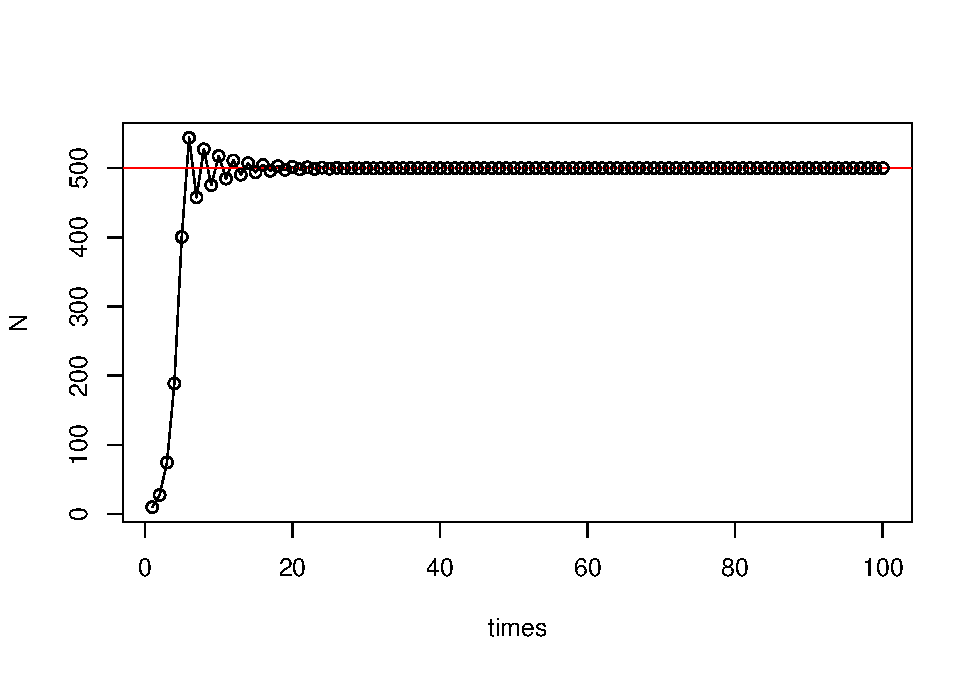
\includegraphics{bookdown-demo_files/figure-latex/unnamed-chunk-15-1.pdf}

\hypertarget{week-4---discrete-exponential-and-logistic-models}{%
\chapter*{Week 4 - Discrete exponential and logistic models}\label{week-4---discrete-exponential-and-logistic-models}}
\addcontentsline{toc}{chapter}{Week 4 - Discrete exponential and logistic models}

\textbf{Part 1 - Model the discrete logistic population growth using for loops}
Model:
\[
N_{t+1} = N_t(1+r(1-\frac{N_t}{K}))
\]

\begin{Shaded}
\begin{Highlighting}[]
\DocumentationTok{\#\#\# (1) Define the discrete logistic growth equation}
\NormalTok{log\_fun }\OtherTok{\textless{}{-}} \ControlFlowTok{function}\NormalTok{(r, N, K)\{N }\SpecialCharTok{+}\NormalTok{ r}\SpecialCharTok{*}\NormalTok{N}\SpecialCharTok{*}\NormalTok{(}\DecValTok{1}\SpecialCharTok{{-}}\NormalTok{N}\SpecialCharTok{/}\NormalTok{K)\}}
\end{Highlighting}
\end{Shaded}

You may modify \(r\) to see the change in stability of equilibrium \(K\).

\begin{Shaded}
\begin{Highlighting}[]
\DocumentationTok{\#\#\# (2) Set the parameters}
\NormalTok{r }\OtherTok{\textless{}{-}} \FloatTok{1.8}
\NormalTok{K }\OtherTok{\textless{}{-}} \DecValTok{500}
\NormalTok{N0 }\OtherTok{\textless{}{-}} \DecValTok{10}
\NormalTok{time }\OtherTok{\textless{}{-}} \DecValTok{100}

\NormalTok{Parms }\OtherTok{\textless{}{-}} \FunctionTok{c}\NormalTok{(}\AttributeTok{r =}\NormalTok{ r, }\AttributeTok{K =}\NormalTok{ K)}

\DocumentationTok{\#\#\# (3) Use for loop to iterate over the time sequence}
\NormalTok{pop\_size }\OtherTok{\textless{}{-}} \FunctionTok{data.frame}\NormalTok{(}\AttributeTok{times =} \DecValTok{1}\SpecialCharTok{:}\NormalTok{time)}
\NormalTok{pop\_size}\SpecialCharTok{$}\NormalTok{N[}\DecValTok{1}\NormalTok{] }\OtherTok{\textless{}{-}}\NormalTok{ N0}

\ControlFlowTok{for}\NormalTok{(i }\ControlFlowTok{in} \DecValTok{2}\SpecialCharTok{:}\NormalTok{time)\{}
\NormalTok{  pop\_size}\SpecialCharTok{$}\NormalTok{N[i] }\OtherTok{\textless{}{-}} \FunctionTok{log\_fun}\NormalTok{(}\AttributeTok{r =}\NormalTok{ r, }\AttributeTok{N =}\NormalTok{ pop\_size}\SpecialCharTok{$}\NormalTok{N[i }\SpecialCharTok{{-}} \DecValTok{1}\NormalTok{], }\AttributeTok{K =}\NormalTok{ K)}
\NormalTok{\}}

\DocumentationTok{\#\#\# (4) Population trajectory}
\FunctionTok{plot}\NormalTok{(N }\SpecialCharTok{\textasciitilde{}}\NormalTok{ times, }\AttributeTok{data =}\NormalTok{ pop\_size, }\AttributeTok{type =} \StringTok{"l"}\NormalTok{)}
\FunctionTok{abline}\NormalTok{(}\AttributeTok{h =}\NormalTok{ K, }\AttributeTok{col =} \StringTok{"red"}\NormalTok{)}
\FunctionTok{points}\NormalTok{(N }\SpecialCharTok{\textasciitilde{}}\NormalTok{ times, }\AttributeTok{data =}\NormalTok{ pop\_size)}
\end{Highlighting}
\end{Shaded}

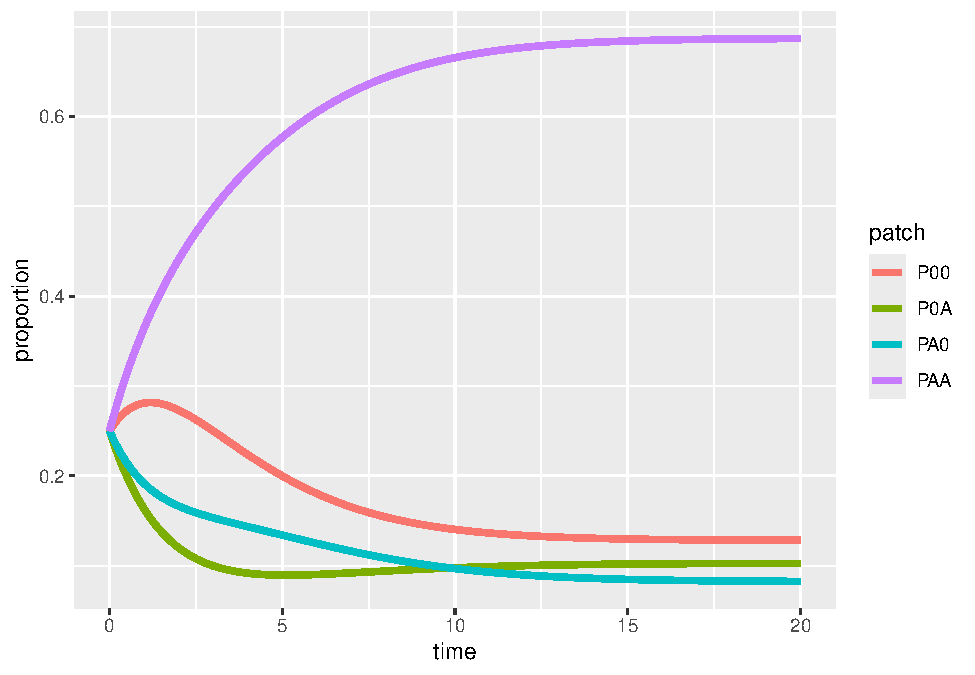
\includegraphics{bookdown-demo_files/figure-latex/unnamed-chunk-17-1.pdf}

\textbf{Part 2 - Generic cobweb}

\begin{Shaded}
\begin{Highlighting}[]
\DocumentationTok{\#\#\#\#\#\# Part 2: Generic cobweb}
\DocumentationTok{\#\#\# (1) define function}
\NormalTok{ReturnMap }\OtherTok{\textless{}{-}} \ControlFlowTok{function}\NormalTok{(Func, x0, times, xmax, }\AttributeTok{curve\_n =} \DecValTok{1000}\NormalTok{, parms)\{}
  
  \CommentTok{\# get time series iteration}
\NormalTok{  x }\OtherTok{\textless{}{-}} \FunctionTok{rep}\NormalTok{(x0, times)}
  \ControlFlowTok{for}\NormalTok{(i }\ControlFlowTok{in} \DecValTok{2}\SpecialCharTok{:}\NormalTok{times)\{}
\NormalTok{    x[i] }\OtherTok{\textless{}{-}} \FunctionTok{Func}\NormalTok{(x[i}\DecValTok{{-}1}\NormalTok{], parms)}
\NormalTok{  \}}
  
  \CommentTok{\# get fine grid for function curve}
\NormalTok{  x.grid }\OtherTok{\textless{}{-}} \FunctionTok{seq}\NormalTok{(}\DecValTok{0}\NormalTok{, xmax, }\AttributeTok{length.out =}\NormalTok{ curve\_n)}
\NormalTok{  y.grid }\OtherTok{\textless{}{-}} \FunctionTok{Func}\NormalTok{(x.grid, parms)}
\NormalTok{  ymax }\OtherTok{\textless{}{-}} \FunctionTok{max}\NormalTok{(y.grid, xmax)}
  
  \CommentTok{\# create canvas}
  \FunctionTok{plot}\NormalTok{(}\ConstantTok{NA}\NormalTok{, }\AttributeTok{xlim =} \FunctionTok{c}\NormalTok{(}\DecValTok{0}\NormalTok{, xmax), }\AttributeTok{ylim =} \FunctionTok{c}\NormalTok{(}\DecValTok{0}\NormalTok{, ymax), }\AttributeTok{xaxs =} \StringTok{"i"}\NormalTok{, }\AttributeTok{yaxs =} \StringTok{"i"}\NormalTok{, }\AttributeTok{bty =} \StringTok{"l"}\NormalTok{, }
       \AttributeTok{xlab =} \FunctionTok{expression}\NormalTok{(N[t]), }\AttributeTok{ylab =} \FunctionTok{expression}\NormalTok{(N[t}\SpecialCharTok{+}\DecValTok{1}\NormalTok{]))}
  \FunctionTok{abline}\NormalTok{(}\AttributeTok{a =} \DecValTok{0}\NormalTok{, }\AttributeTok{b =} \DecValTok{1}\NormalTok{, }\AttributeTok{lty =} \DecValTok{2}\NormalTok{, }\AttributeTok{col =} \StringTok{"grey50"}\NormalTok{)          }
  \FunctionTok{lines}\NormalTok{(x.grid, y.grid, }\AttributeTok{col =} \StringTok{"steelblue"}\NormalTok{, }\AttributeTok{lwd =} \DecValTok{2}\NormalTok{)      }
  
  \CommentTok{\# cobweb (horizontal to diagonal, vertical up to function)}
  \FunctionTok{segments}\NormalTok{(}\AttributeTok{x0 =}\NormalTok{ x[}\DecValTok{1}\NormalTok{], }\AttributeTok{y0 =} \DecValTok{0}\NormalTok{,   }\AttributeTok{x1 =}\NormalTok{ x[}\DecValTok{1}\NormalTok{],   }\AttributeTok{y1 =}\NormalTok{ x[}\DecValTok{2}\NormalTok{], }\AttributeTok{col =} \StringTok{"firebrick"}\NormalTok{)}
  \ControlFlowTok{for}\NormalTok{(i }\ControlFlowTok{in} \DecValTok{2}\SpecialCharTok{:}\NormalTok{(times}\DecValTok{{-}1}\NormalTok{))\{}
    \FunctionTok{segments}\NormalTok{(}\AttributeTok{x0 =}\NormalTok{ x[i}\DecValTok{{-}1}\NormalTok{], }\AttributeTok{y0 =}\NormalTok{ x[i],   }
             \AttributeTok{x1 =}\NormalTok{ x[i],   }\AttributeTok{y1 =}\NormalTok{ x[i], }\AttributeTok{col =} \StringTok{"firebrick"}\NormalTok{)}
    \FunctionTok{segments}\NormalTok{(}\AttributeTok{x0 =}\NormalTok{ x[i],   }\AttributeTok{y0 =}\NormalTok{ x[i], }
             \AttributeTok{x1 =}\NormalTok{ x[i],   }\AttributeTok{y1 =}\NormalTok{ x[i}\SpecialCharTok{+}\DecValTok{1}\NormalTok{], }\AttributeTok{col =} \StringTok{"firebrick"}\NormalTok{)}
\NormalTok{  \}}
  
\NormalTok{\}}

\DocumentationTok{\#\#\# (2) Set up different discrete model function with outside parameters}

\DocumentationTok{\#\#\#\# Discrete logistic function with outside parameters}
\NormalTok{Logistic }\OtherTok{\textless{}{-}} \ControlFlowTok{function}\NormalTok{(N, parms)\{}
  \FunctionTok{with}\NormalTok{(}\FunctionTok{as.list}\NormalTok{(parms), \{}
    \FunctionTok{return}\NormalTok{(N }\SpecialCharTok{+}\NormalTok{ r}\SpecialCharTok{*}\NormalTok{N}\SpecialCharTok{*}\NormalTok{(}\DecValTok{1}\SpecialCharTok{{-}}\NormalTok{N}\SpecialCharTok{/}\NormalTok{K))}
\NormalTok{  \})}
\NormalTok{\}}
\NormalTok{Parms }\OtherTok{\textless{}{-}} \FunctionTok{c}\NormalTok{(}\AttributeTok{r =}\NormalTok{ r, }\AttributeTok{K =}\NormalTok{ K)}

\DocumentationTok{\#\#\#\# Ricker function with outside parameters}
\NormalTok{Ricker }\OtherTok{\textless{}{-}} \ControlFlowTok{function}\NormalTok{(N, parms)\{}
  \FunctionTok{with}\NormalTok{(}\FunctionTok{as.list}\NormalTok{(parms), \{}
    \FunctionTok{return}\NormalTok{(N }\SpecialCharTok{*} \FunctionTok{exp}\NormalTok{(r}\SpecialCharTok{*}\NormalTok{(}\DecValTok{1}\SpecialCharTok{{-}}\NormalTok{N}\SpecialCharTok{/}\NormalTok{K)))}
\NormalTok{  \})}
\NormalTok{\}}
\NormalTok{Parms }\OtherTok{\textless{}{-}} \FunctionTok{c}\NormalTok{(}\AttributeTok{r =}\NormalTok{ r, }\AttributeTok{K =}\NormalTok{ K)}

\DocumentationTok{\#\#\#\# Beverton{-}Holt function with outside parameters}
\NormalTok{Beverton }\OtherTok{\textless{}{-}} \ControlFlowTok{function}\NormalTok{(N, parms)\{}
  \FunctionTok{with}\NormalTok{(}\FunctionTok{as.list}\NormalTok{(parms), \{}
    \FunctionTok{return}\NormalTok{(lambda }\SpecialCharTok{*}\NormalTok{ N }\SpecialCharTok{/}\NormalTok{ (}\DecValTok{1} \SpecialCharTok{+}\NormalTok{ alpha }\SpecialCharTok{*}\NormalTok{ N))}
\NormalTok{  \})}
\NormalTok{\}}
\NormalTok{Parms }\OtherTok{\textless{}{-}} \FunctionTok{c}\NormalTok{(}\AttributeTok{lambda =} \FloatTok{1.2}\NormalTok{, }\AttributeTok{alpha =} \FloatTok{0.2}\NormalTok{)}


\DocumentationTok{\#\#\# (3) Use the ReturnMap function}

\FunctionTok{ReturnMap}\NormalTok{(}\AttributeTok{Func =}\NormalTok{ Logistic,}
          \AttributeTok{x0 =} \DecValTok{10}\NormalTok{, }
          \AttributeTok{times =} \DecValTok{150}\NormalTok{,}
          \AttributeTok{xmax =} \DecValTok{310}\NormalTok{,}
          \AttributeTok{curve\_n =} \DecValTok{1000}\NormalTok{, }
          \AttributeTok{parms =}\NormalTok{ Parms)}
\end{Highlighting}
\end{Shaded}

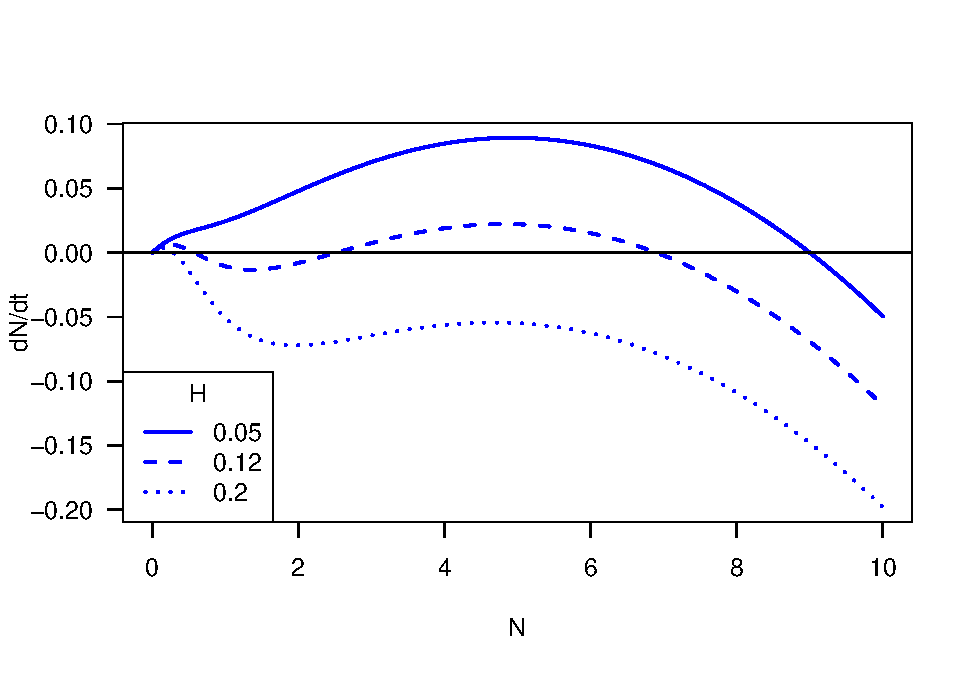
\includegraphics{bookdown-demo_files/figure-latex/unnamed-chunk-18-1.pdf}

Here is a shiny app for the discrete logistic growth model.

Credit to \href{https://genchanghsu.github.io/index.html}{Gen-Chang Hsu}

\textbf{Part 3 - Bifurcation}

\begin{Shaded}
\begin{Highlighting}[]
\DocumentationTok{\#\#\#\#\# Part 3: Logistic map and bifurcation}

\DocumentationTok{\#\#\# (1) Define the function}
\NormalTok{RickerPlot }\OtherTok{\textless{}{-}} \ControlFlowTok{function}\NormalTok{(Func, variable, var\_vec, x0, times, }\AttributeTok{x\_print =} \DecValTok{200}\NormalTok{, parms)\{}
  
  \CommentTok{\# prepare saving space }
\NormalTok{  data\_plot }\OtherTok{\textless{}{-}} \FunctionTok{data.frame}\NormalTok{(}\AttributeTok{var =} \FunctionTok{rep}\NormalTok{(var\_vec, }\AttributeTok{each =}\NormalTok{ x\_print), }\AttributeTok{x =} \DecValTok{0}\NormalTok{)}
  
  \CommentTok{\# change bifurcation parameter}
  \ControlFlowTok{for}\NormalTok{ (k }\ControlFlowTok{in} \DecValTok{1}\SpecialCharTok{:}\FunctionTok{length}\NormalTok{(var\_vec))\{}
\NormalTok{    parms[variable] }\OtherTok{\textless{}{-}}\NormalTok{ var\_vec[k]}
\NormalTok{    x }\OtherTok{\textless{}{-}} \FunctionTok{rep}\NormalTok{(x0, times)}
    
    \CommentTok{\# get time series with new bifurcation parameter}
    \ControlFlowTok{for}\NormalTok{(i }\ControlFlowTok{in} \DecValTok{2}\SpecialCharTok{:}\NormalTok{times)\{}
\NormalTok{      x[i] }\OtherTok{\textless{}{-}} \FunctionTok{Func}\NormalTok{(x[i}\DecValTok{{-}1}\NormalTok{], parms)}
\NormalTok{    \}}
    
    \CommentTok{\# save the data}
\NormalTok{    data\_plot}\SpecialCharTok{$}\NormalTok{x[(}\DecValTok{1} \SpecialCharTok{+}\NormalTok{ (k }\SpecialCharTok{{-}} \DecValTok{1}\NormalTok{)}\SpecialCharTok{*}\NormalTok{x\_print)}\SpecialCharTok{:}\NormalTok{(k}\SpecialCharTok{*}\NormalTok{x\_print)] }\OtherTok{\textless{}{-}}\NormalTok{ x[(times }\SpecialCharTok{{-}}\NormalTok{ x\_print }\SpecialCharTok{+} \DecValTok{1}\NormalTok{)}\SpecialCharTok{:}\NormalTok{times]}
\NormalTok{  \}}
  
  \CommentTok{\# plot }
  \FunctionTok{plot}\NormalTok{(x }\SpecialCharTok{\textasciitilde{}}\NormalTok{ var, }\AttributeTok{data =}\NormalTok{ data\_plot, }\AttributeTok{cex =} \FloatTok{0.05}\NormalTok{, }\AttributeTok{pch =} \DecValTok{20}\NormalTok{, }
       \AttributeTok{xlab =}\NormalTok{ variable, }\AttributeTok{ylab =} \StringTok{"Population size"}\NormalTok{)}
  
\NormalTok{\}}

\DocumentationTok{\#\#\#\# Discrete logistic function with outside parameters}
\NormalTok{Logistic }\OtherTok{\textless{}{-}} \ControlFlowTok{function}\NormalTok{(N, parms)\{}
  \FunctionTok{with}\NormalTok{(}\FunctionTok{as.list}\NormalTok{(parms), \{}
    \FunctionTok{return}\NormalTok{(N }\SpecialCharTok{+}\NormalTok{ r}\SpecialCharTok{*}\NormalTok{N}\SpecialCharTok{*}\NormalTok{(}\DecValTok{1}\SpecialCharTok{{-}}\NormalTok{N}\SpecialCharTok{/}\NormalTok{K))}
\NormalTok{  \})}
\NormalTok{\}}

\DocumentationTok{\#\#\# (2) Parameter setting}

\NormalTok{Parms }\OtherTok{\textless{}{-}} \FunctionTok{c}\NormalTok{(}\AttributeTok{r =}\NormalTok{ r, }\AttributeTok{K =}\NormalTok{ K)}
\NormalTok{r\_seq }\OtherTok{\textless{}{-}} \FunctionTok{seq}\NormalTok{(}\AttributeTok{from =} \FloatTok{1.8}\NormalTok{, }\AttributeTok{to =} \DecValTok{3}\NormalTok{, }\AttributeTok{by =} \FloatTok{0.001}\NormalTok{)}

\DocumentationTok{\#\#\# (3) Use generic ricker plot function}
\FunctionTok{RickerPlot}\NormalTok{(}\AttributeTok{Func =}\NormalTok{ Logistic, }
           \AttributeTok{variable =} \StringTok{"r"}\NormalTok{, }
           \AttributeTok{var\_vec =}\NormalTok{ r\_seq, }
           \AttributeTok{x0 =} \DecValTok{10}\NormalTok{, }
           \AttributeTok{times =} \DecValTok{500}\NormalTok{, }
           \AttributeTok{x\_print =} \DecValTok{100}\NormalTok{, }
           \AttributeTok{parms =}\NormalTok{ Parms)}
\end{Highlighting}
\end{Shaded}

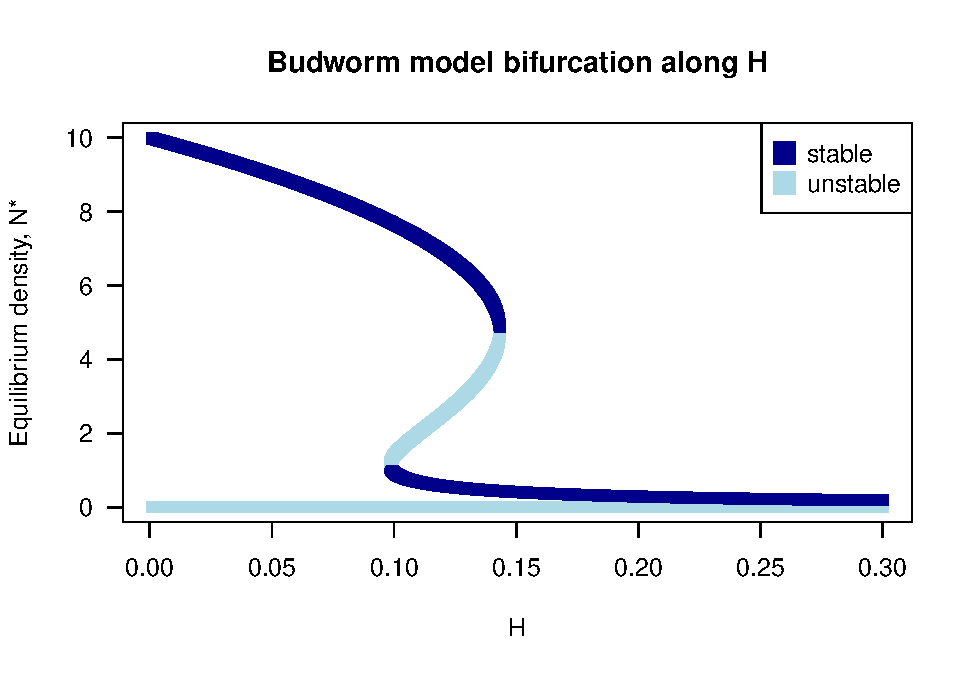
\includegraphics{bookdown-demo_files/figure-latex/unnamed-chunk-20-1.pdf}

  \bibliography{book.bib,packages.bib}

\end{document}
